\clearpage
\VerdierPhysicalPageAnchor{0140}%
\begingroup
\normalsize
\setlength{\parskip}{0pt}%
\setlength{\emergencystretch}{1.5em}%
\setlength{\abovedisplayskip}{1pt plus 1pt minus 1pt}%
\setlength{\belowdisplayskip}{1pt plus 1pt minus 1pt}%

\VerdierSemanticAnchor{ch2-2-2-6-proof-b-triii-completion}
\noindent が与えられたとき、$(m,p,r)$ が三角の射となるような射
$r\colon Q(Z)\longrightarrow Q(Z')$ が存在する。
\VerdierSemanticAnchor{ch2-2-2-6-proof-b-triii-case-reduction}%
補題 (2.2.7) により、次の二つの場合を考えればよい：

\VerdierSemanticAnchor{ch2-2-2-6-proof-b-triii-case-a}
\noindent\textit{a)}\quad
$m=Q(s)^{-1}$、$p=Q(t)^{-1}$、$s,t\in S$ であり、図式

\VerdierSemanticAnchor{ch2-2-2-6-proof-b-triii-case-a-square}
\begin{center}
  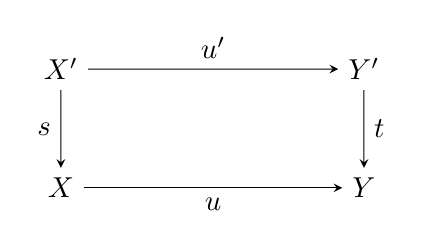
\begin{tikzpicture}[>=stealth,line width=.38pt,x=1.85cm,y=1.45cm,
    scale=1.04,transform shape]
    \node (Xp) at (0,1) {$X'$};
    \node (Yp) at (2,1) {$Y'$};
    \node (X)  at (0,0) {$X$};
    \node (Y)  at (2,0) {$Y$};
    \draw[->] (Xp) -- node[above] {$u'$} (Yp);
    \draw[->] (Xp) -- node[left] {$s$} (X);
    \draw[->] (Yp) -- node[right] {$t$} (Y);
    \draw[->] (X) -- node[below] {$u$} (Y);
  \end{tikzpicture}
\end{center}

\noindent は可換である。

\VerdierSemanticAnchor{ch2-2-2-6-proof-b-triii-case-b}
\noindent\textit{b)}\quad
$m=Q(f)$、$p=Q(g)$ であり、図式

\VerdierSemanticAnchor{ch2-2-2-6-proof-b-triii-case-b-square}
\begin{center}
  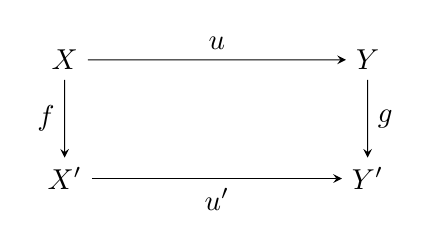
\begin{tikzpicture}[>=stealth,line width=.38pt,x=1.85cm,y=1.45cm,
    scale=1.04,transform shape]
    \node (X)  at (0,1) {$X$};
    \node (Y)  at (2,1) {$Y$};
    \node (Xp) at (0,0) {$X'$};
    \node (Yp) at (2,0) {$Y'$};
    \draw[->] (X) -- node[above] {$u$} (Y);
    \draw[->] (X) -- node[left] {$f$} (Xp);
    \draw[->] (Y) -- node[right] {$g$} (Yp);
    \draw[->] (Xp) -- node[below] {$u'$} (Yp);
  \end{tikzpicture}
\end{center}

\noindent は可換である。

\VerdierSemanticAnchor{ch2-2-2-6-proof-b-triii-case-conclusion}
\noindent 場合 \textit{a)} では、主張は性質 SM6) (2.1.2) から従う。
場合 \textit{b)} では、$\mathcal D$ の完全三角に対する性質 TRIII から
従う。

\VerdierSemanticAnchor{ch2-2-2-8}
\smallskip
\noindent\textbf{2.2.8.\quad 補題 2.2.7 の証明。}
\VerdierSemanticAnchor{ch2-2-2-8-initial-lift}%
定理 (2.2.2) により、$pQ(t)=Q(g)$ を満たす射
$t\colon Y''\longrightarrow Y$、$t\in S$ が存在する。ただし
$g\colon Y''\longrightarrow Y'$ である。次の図式を段階的に構成する：

\VerdierSemanticAnchor{ch2-2-2-8-stepwise-diagram}
\begin{center}
  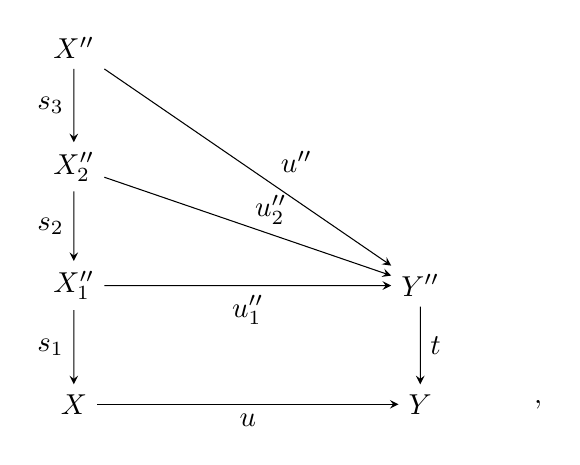
\begin{tikzpicture}[>=stealth,line width=.38pt,x=1.80cm,y=1.45cm,
    scale=1.04,transform shape]
    \node (Xpp)  at (0,3) {$X''$};
    \node (X2pp) at (0,2) {$X_2''$};
    \node (X1pp) at (0,1) {$X_1''$};
    \node (X)    at (0,0) {$X$};
    \node (Ypp)  at (2.35,1) {$Y''$};
    \node (Y)    at (2.35,0) {$Y$};
    \draw[->] (Xpp) -- node[left] {$s_3$} (X2pp);
    \draw[->] (X2pp) -- node[left] {$s_2$} (X1pp);
    \draw[->] (X1pp) -- node[left] {$s_1$} (X);
    \draw[->] (Xpp) -- node[pos=.58,above right] {$u''$} (Ypp);
    \draw[->] (X2pp) -- node[pos=.58,above] {$u_2''$} (Ypp);
    \draw[->] (X1pp) -- node[below] {$u_1''$} (Ypp);
    \draw[->] (Ypp) -- node[right] {$t$} (Y);
    \draw[->] (X) -- node[below] {$u$} (Y);
    \node at (3.15,0) {$,$};
  \end{tikzpicture}
\end{center}

\VerdierSemanticAnchor{ch2-2-2-8-proof-p141-boundary}
\VerdierSemanticAnchor{ch2-2-2-8-p141-boundary}
\endgroup
